\documentclass{article}

% Language setting
% Replace `english' with e.g. `spanish' to change the document language
\usepackage[english]{babel}

% Set page size and margins
% Replace `letterpaper' with `a4paper' for UK/EU standard size
\usepackage[letterpaper,top=2cm,bottom=2cm,left=3cm,right=3cm,marginparwidth=1.75cm]{geometry}

% Useful packages
\usepackage{amsmath}
\usepackage{graphicx}
\usepackage{subcaption}
\usepackage{enumitem}
\usepackage[colorlinks=true, allcolors=blue]{hyperref}
\usepackage{longtable}
\usepackage{appendix}

\title{SongSwipe}
\author{Christopher Coco, Nena Heng, Raj Ray, Anthony Simao, Katiana Sourn}

\begin{document}
\maketitle

\begin{abstract}
SongSwipe is a web application that allows for an easier, quicker, and more user friendly experience of managing a Spotify playlist. It allows for a simple Tinder-inspired swipe left-or-right motion to decide whether a song will remain in your playlist or be removed. Previews of the song will be played automatically. Not only can a user easily remove unwanted old songs from their own playlists, but also filter out songs from a copy of another user's playlist to make it more personal to the user.
\end{abstract}

\section{The Problem}
With over 250 million users and 31.7\% of the music streaming platform market share \cite{Spotify_stats}, Spotify \cite{Spotify_app} has revolutionized how we access and enjoy music. Over the years, Spotify's user interface has gone through numerous changes and redesigns, many of which have been met with frustration. One of the most notable changes was the remapping of playlist functions and buttons, leaving many users confused as they felt there was no need to fix what wasn’t broken. Despite its unpopularity, the change remains in effect to this day, leaving the process of managing playlists, a cumbersome one.\\

Over time, playlists tend to become bloated with songs that were once enjoyed by the user, but are now often skipped over. Many users find themselves wanting to update their playlists. Unfortunately, Spotify offers no easy or convenient solution to do this, and removing unwanted songs from a playlist is a tedious process that gets more frustrating the more times a user has to do it, the steps are:
\begin{enumerate}
  \item Click the playlist button in the bottom right corner.
  \begin{itemize}
    \item[$\rightarrow$] This opens a list of all playlists the current song is in.
  \end{itemize}

  \item Uncheck the playlist you want the song removed from.
  \begin{itemize}
    \item[$\rightarrow$] This will remove the current song from that specific playlist.
  \end{itemize}

  \item Click the done button in the bottom center.
  \begin{itemize}
    \item[$\rightarrow$] This will return you to the now playing screen.
  \end{itemize}

  \item Swipe to the next song and repeat.
  \begin{itemize}
    \item[$\rightarrow$] Repeat until all unwanted songs are removed.
  \end{itemize}
\end{enumerate}

\begin{figure}[ht]
  \centering
  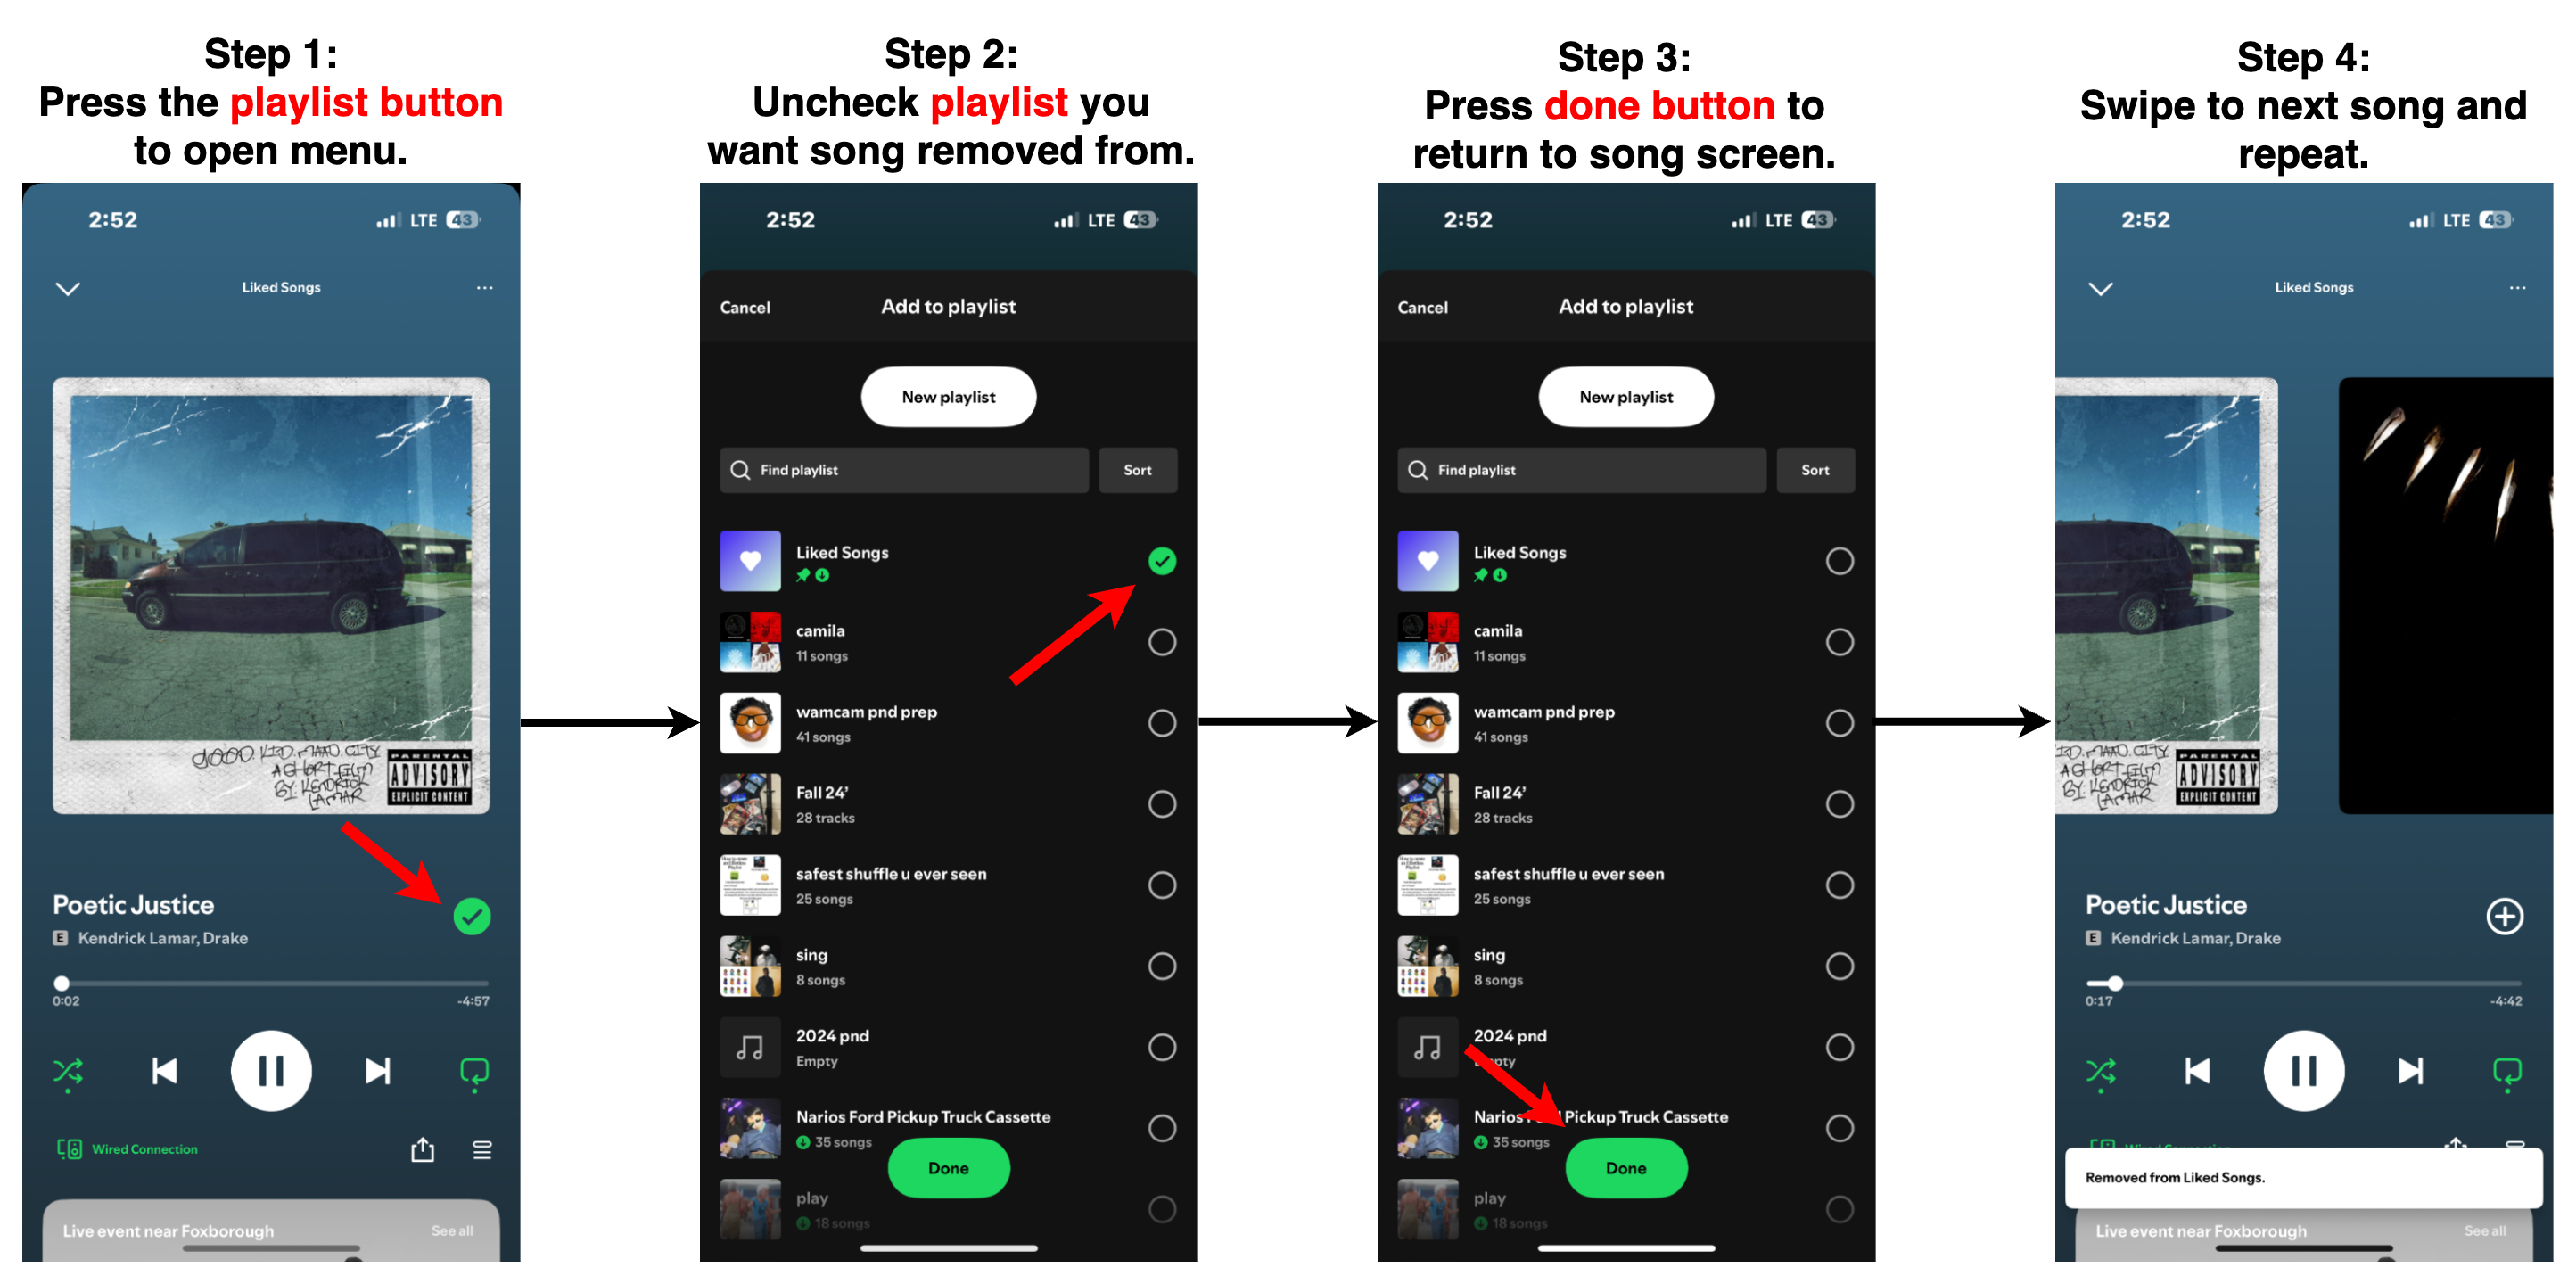
\includegraphics[width=\textwidth]{./spotify_diagram.png}
  \caption{The steps it takes to remove a song from a playlist.}
  \label{fig:spotify_diagram}
\end{figure}


% \begin{center}
%     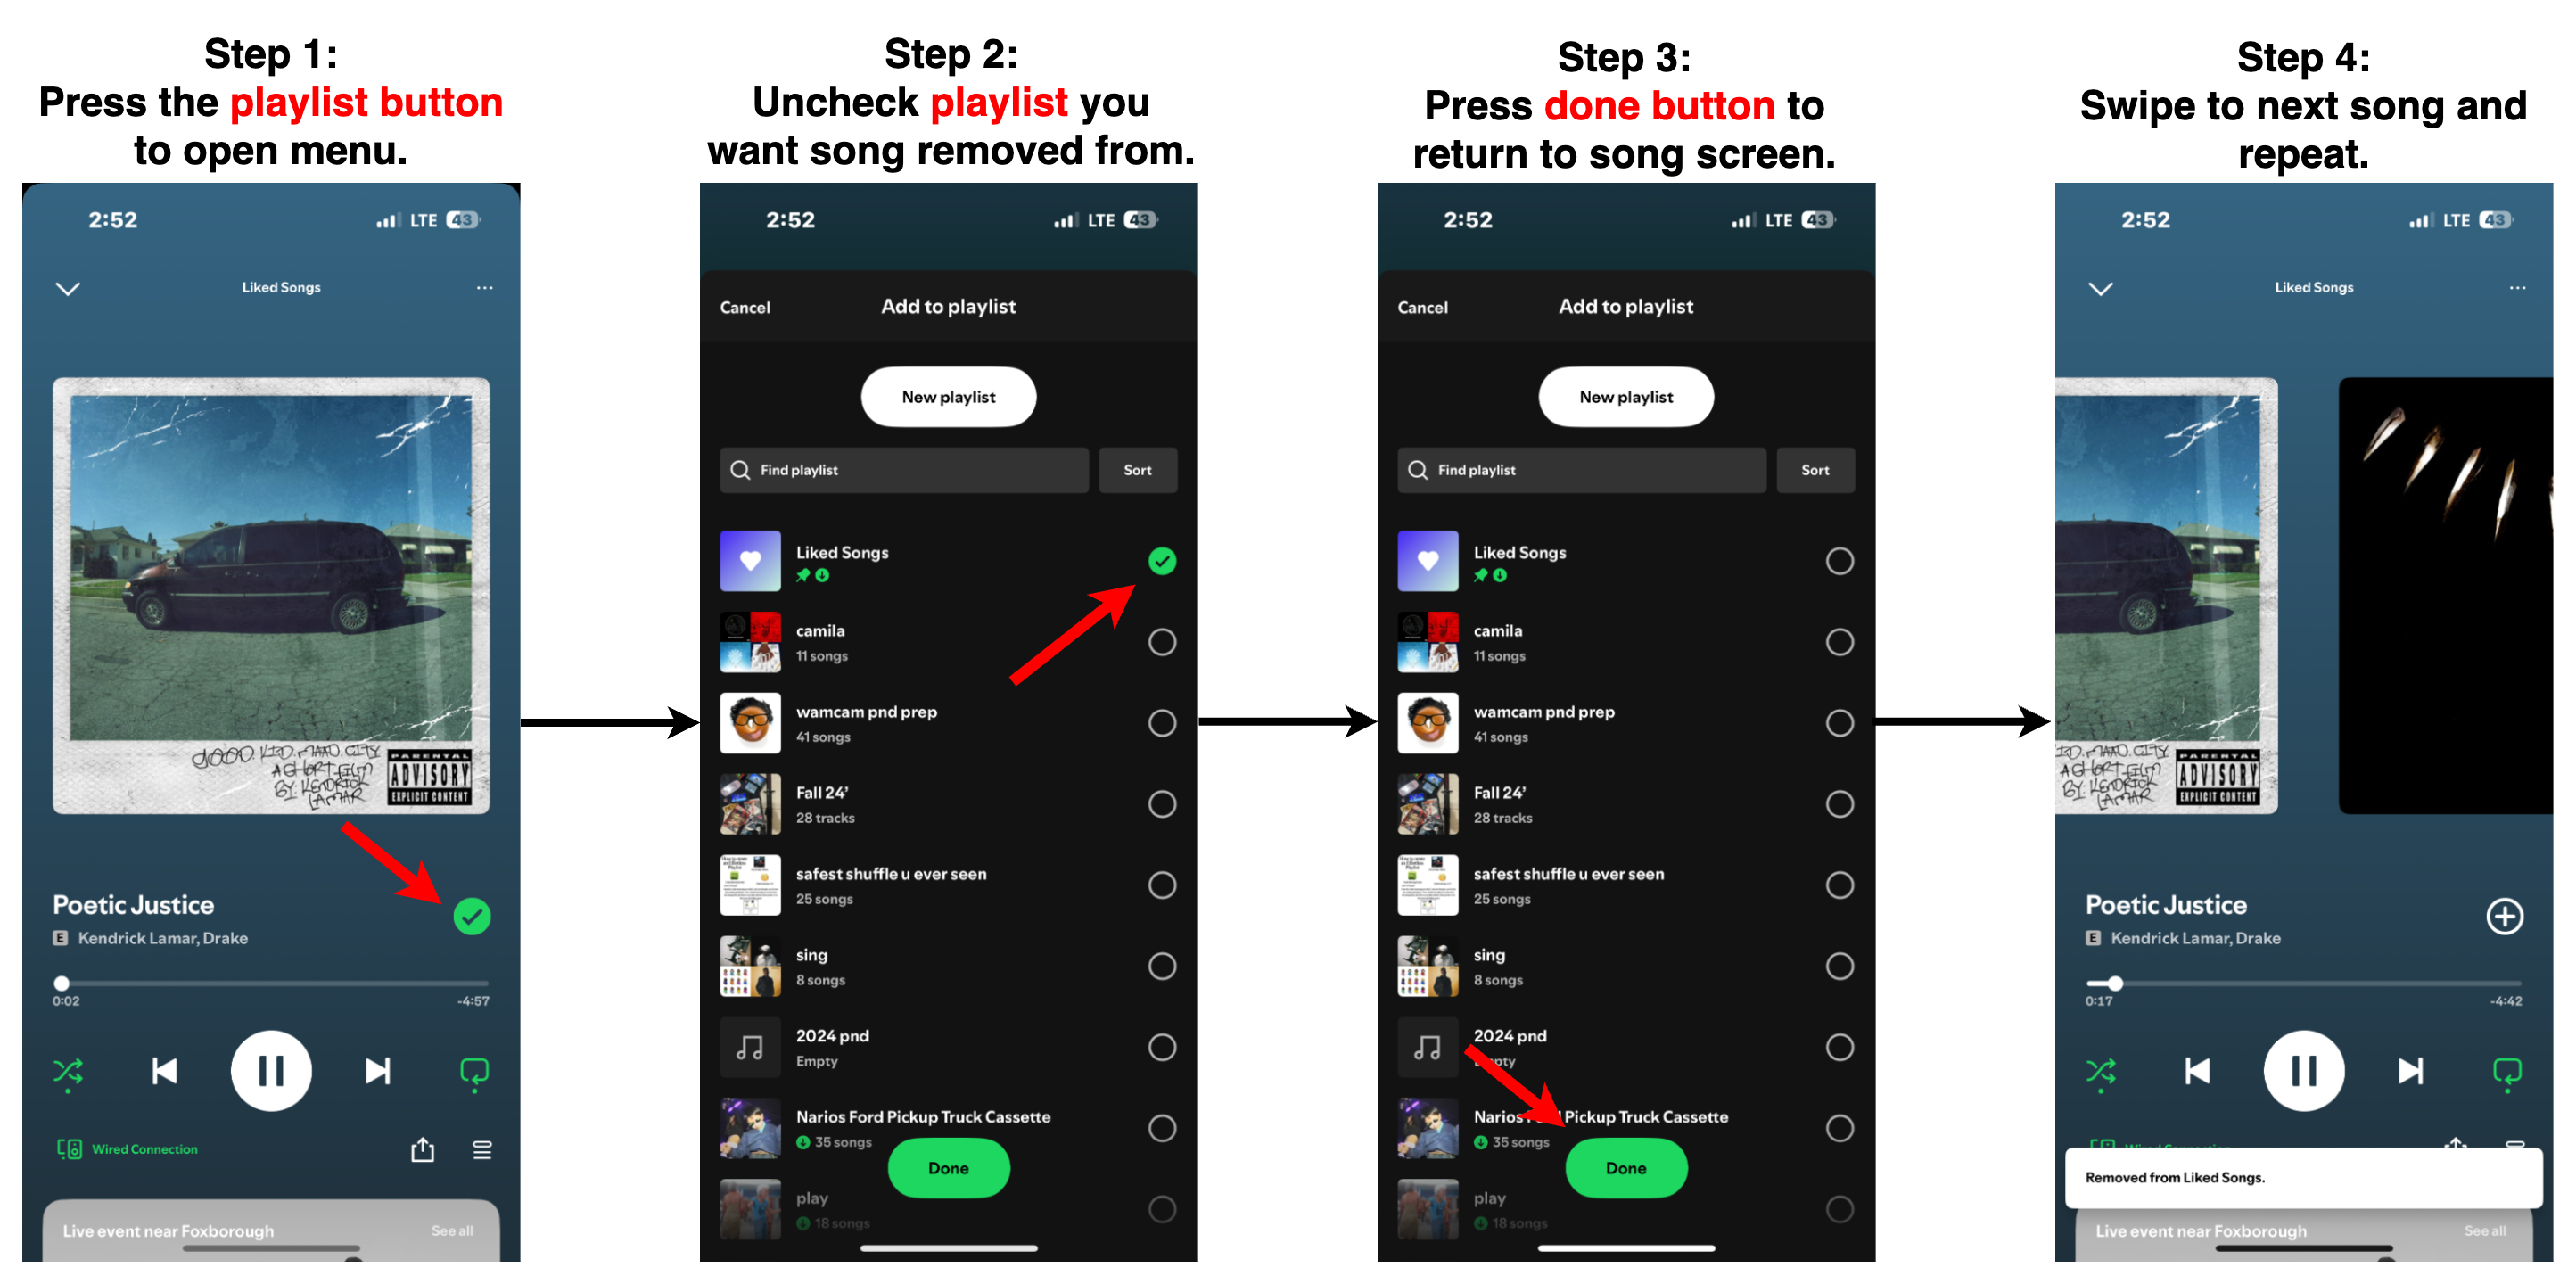
\includegraphics[width=15cm]{spotify_diagram.png}
% \end{center}


With each song removed costing 3 button presses, removing 100 songs would require at least 300 button presses in combination with swiping between each track.  In combination with the time requirement of listen to song introductions, the process is both time-consuming and frustrating.  This single design flaw further tarnishes the overall user experience, as users end up skipping songs repeatedly.  Spotify also allows users to copy existing playlists created by other users to one's own library.  Yet many people do not use this feature as there is no way to easily remove the songs that they don’t like from the copied playlist.\\

\section{Current Solutions}
Many Spotify users struggle with the platform's limited playlist management features. People change and so do their music preferences. Spotify’s inefficient platform makes it difficult for users to keep playlists organized and up to date.\\

Spotify's platform is lacking in playlist management such as efficient revision of playlists. Some users end up creating a new playlist of what they currently like, as it is seen as a better alternative, which causes users to have a cluttered Spotify library filled with many playlist. While Spotify\'s built-in playlist management is limited, several external tools have emerged such as Spotify Dedup, Playmixify, Swipefy, and Skiley.net.

\subsection{Spotify Dedup}
\quad Spotify Dedup is a web app that analyzes your library and removes duplicates. It uses the Spotify API and links to access your account. Its simple UI shows your playlist that contains duplicates, details of the artist, and song: and then the option to remove duplicates from your playlist. \cite{Spotify_dedup} The web app Spotify Dedup is successful as it is very direct about its approach - simple UI and simple function. On the other hand, that is all it will do. What makes our product better than Spotify Dedup is that we will allow you to not only remove duplicates, but also have an interactive UI that makes managing a playlist less tedious and more entertaining. 

\begin{figure}[ht]
  \centering
  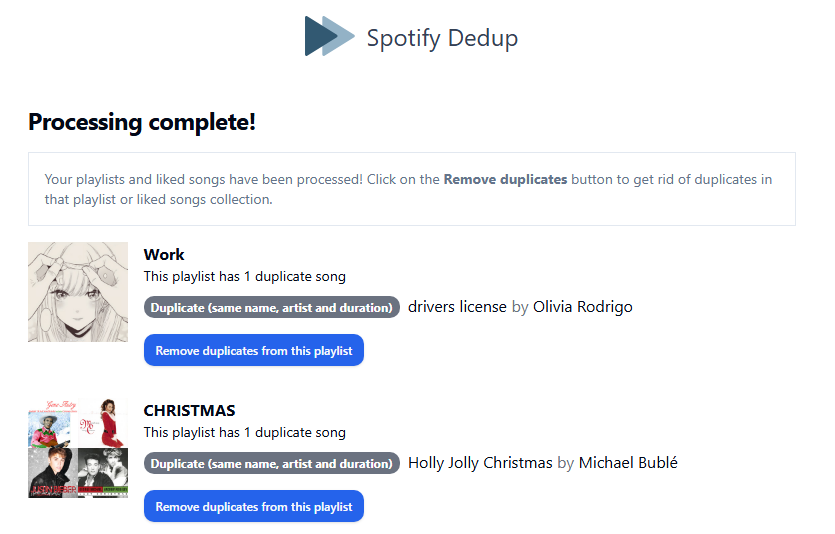
\includegraphics[width=\textwidth]{./dedupss.png}
  \caption{The Spotify Dedup desktop GUI.}
  \label{fig:dedup}
\end{figure}

\pagebreak

\subsection{Playmixify}
\quad Playmixify is a web application that ``mixes your Spotify playlists into an ultimate playlist and keeps them in sync with the original playlists`` \cite{Spotify_app}. This application allows you to combine playlists from your library into one massive playlist. It uses the Spotify API to view your library and make a playlist from existing songs in your playlist. Like Spotify Dedup, it is very direct and simple in its approach but just like Dedup - that is all it does. Our product is distinguished from other external tools by offering a more interactive experience with a wider range of playlist management features, going beyond just creating or deleting specific types of playlists.

\begin{figure}[ht]
  \centering
  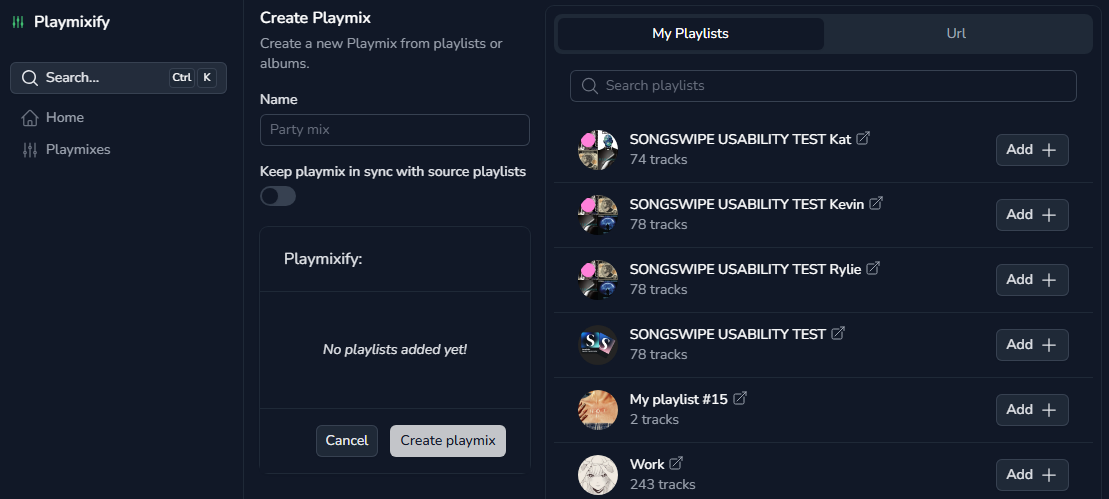
\includegraphics[width=5 in]{./playmixifyss.png}
  \caption{The Playmixify desktop GUI.}
  \label{fig:playmixify}
\end{figure}

\pagebreak

\subsection{Swipefy for Spotify}
\quad Swipefy for Spotify is a mobile app available on IOS and Android that uses the Spotify API to introduce Spotify\'s consumers to new music using an AI algorithm and allows them to seamlessly add these songs to their playlists with an interactive UI - where users can Tinder-Swipe these songs on their app and into their Spotify playlist. \cite{swipefy} Swipefy’s main objective is to introduce songs that the consumer may like based on filters that you can access in the UI and based on similar songs found in a playlist that the consumer wishes to add to. The Swipefy for Spotify is successful in its approach by making an interactive way to allow Spotify consumers to discover new music that is curated for them by using the information found in their profile and playlist. \\

One issue with Swipefy for Spotify is that it is only available as a mobile app. Our team believes that anyone with access to Spotify - regardless of their device or operating system - should be able to use our tool. Therefore, to ensure access to all Spotify users, our application is not only accessible on iOS, but on most devices with a web browser.

\begin{figure}[ht]
  \centering
  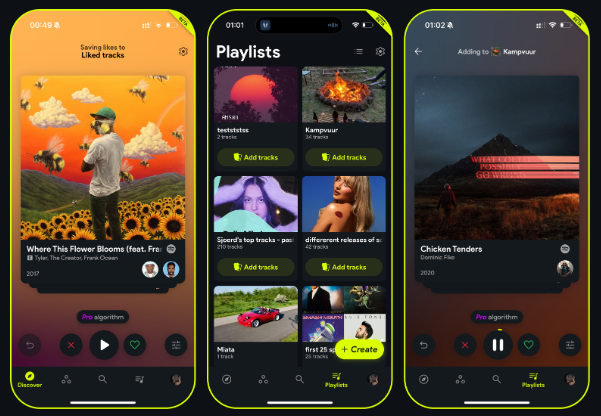
\includegraphics[width=5in]{./swipefyss.png}
  \caption{Samples of Swipefy GUI.}
  \label{fig:swipey}
\end{figure}

\pagebreak

\subsection{Skiley.net}
\quad Skiley.net is a platform that essentially extends the Spotify UI by including numerous features such as song discovery and playlist management. Furthermore, using the Spotify API they replicate the Spotify UI by showing what song you’re listening to, playback history, and the lyrics,  and extend their UI by including additional features such as providing music videos, and similar song recommendations based on the current song you are listening to, and facts associated with the song. They also offer playlist management via deduplication which removes duplicates found in the playlist. \cite{skiley} \\

Although Skiley.net extends the Spotify UI in terms of additional information, they limit playlist management to 3 edits of any of the free service options they provide and offer more services behind a one-time subscription. As Spotify requires consumers to pay a monthly subscription service to remove ads when playing music, it would seem redundant to purchase an external Spotify tool for playlist management and to remove ads from their platform. Furthermore, they provide different ways to organize your playlist, but there still is a lack of an efficient playlist revision tool. \\
\\
\quad SongSwipe has its main focus on revising the playlist revision process to reduce the amount of time it takes revise a playlist, which although Skiley.net has other amazing features, it does not offer the same service we provide.

\begin{figure}[ht]
  \centering
  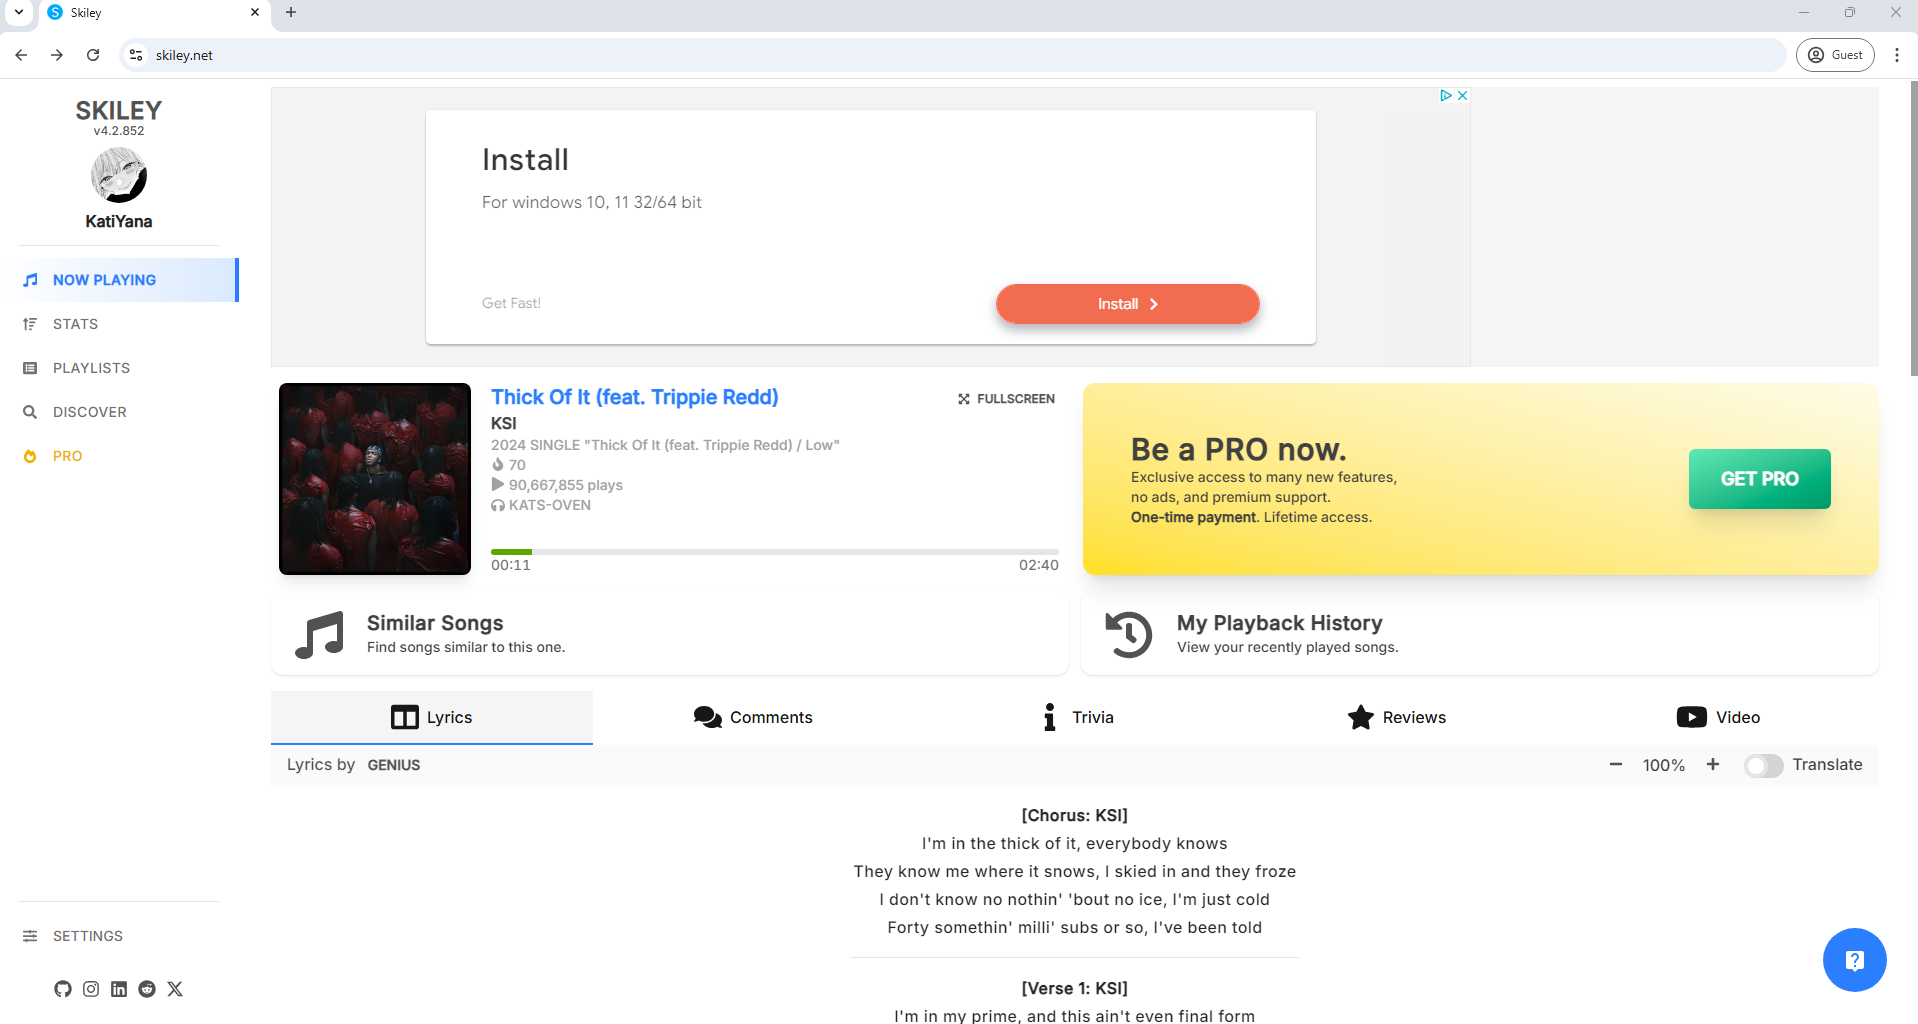
\includegraphics[width=\textwidth]{./skileyss.png}
  \caption{The Skiley desktop GUI.}
  \label{fig:skiley}
\end{figure}

While Spotify is a major platform for music streaming, its playlist management features fail to meet the needs of its users. The current process for managing playlists can be tedious, leading users to create new playlists repeatedly or seek external solutions. Tools like Spotify Dedup, Swipefy for Spotify, Skiley.net, and Playmixify have attempted to address these shortcomings by leveraging the Spotify API to provide additional functionalities such as deduplication, song discovery, and playlist synchronization. However, these tools focus on niche aspects of playlist management and lack of comprehensive, and interactive experience users desire. Our solution will be a discernible tool against other external Spotify tools by offering a free, accessible web app that not only simplifies playlist management but also makes the process more engaging and user-friendly.
 

\section{Our Solution}
\quad The function of our application mainly revolve around managing playlists on Spotify. The user signs into their account so that the application has permission to access user information such as their playlists. This also grants the application permission to manage the user's playlists as well. After selecting a playlist, the user will be brought to a screen that resembles interfaces of dating apps. SongSwipe's main screen has some buttons for playback functionality as well as information about the song including: song title, artist info, and album cover art. When a song is displayed, it will start playing. The user can swipe left on the song if they don't like it, and right if they do. The swiping motions make it easier to select which songs you want to keep or remove.\\

\quad The two playback buttons control both playing and pausing, as well as restarting the current songs preview.  There is also a button to go to the staging area, where all changes live before being commited to Spotify. Each decision the user makes is tracked and saved to the staging area which shows all changes that have been made to the playlist. During or after a user is done going through a playlist, they can see an overview of their changes in this area and then choose to revert any recent changes they have made. After reviewing the staging area and confirming the changes, the application automatically updates the user's Spotify playlist. \\

\quad Another major function of our application is copying playlists from other users. Currently, there is no easy way to copy another user’s playlists on the mobile version of Spotify. Our application improves user satisfaction by allowing consumers to search for a user to copy a playlist from or providing the playlist URL if the playlist is public. Once the consumer copies a playlist, they can use the functions just described to help manage the playlist and adjust it to their liking.

\quad Our solution differs from the existing solutions through a highly navigable and intuitive user interface. The UI is inspired by dating applications like Tinder. This single swipe replaces what would be three seperate button presses on the Spotify app.  It reduces room for error and decreases the amount of input/time that is needed to remove a song from your playlist.
\\

\quad Being able to play the song’s preview before deciding whether to remove or keep it, is another major improvement that our app achieves. Normally, a user would have to listen to the song from the beginning. However, sometimes songs can have a long introduction before they get to the part where you would be able to determine if it’s worth keeping. The preview for a song on Spotify showcases a part of the song that could be considered the best part of it and playing this preview helps Spotify consumers determine whether they like the song or not in a time-effective manner; rather than have them listen to the whole song from start to finish. This feature helps Spotify consumers manage their playlists in an optimal manner.
\\

% \begin{center}
%     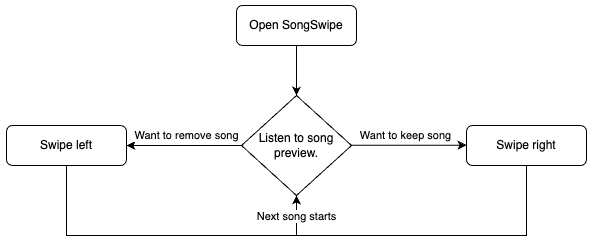
\includegraphics[im stupid]{flow2.png}
% \end{center}

\begin{figure}[h]
    \centering
    \begin{subcaptionbox}{With Spotify's app\label{fig:diagram1}}
        {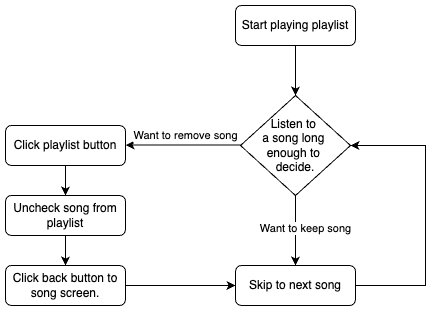
\includegraphics[width=0.60\textwidth]{./flow1.png}}
    \end{subcaptionbox}
    \hspace{1em} % Adjust spacing between images
    \begin{subcaptionbox}{With SongSwipe\label{fig:diagram2}}
        {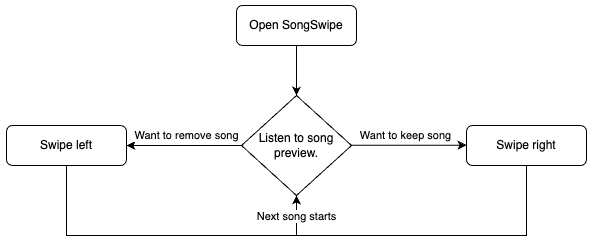
\includegraphics[width=0.75\textwidth]{./flow2.png}}
    \end{subcaptionbox}
    \caption{Flowcharts demonstrating the processes of managing a Spotify playlist.}
    \label{fig:both_diagrams}
\end{figure}

\quad Furthermore, a feature that makes SongSwipe distinguishable from other external Spotify tools is the ability to copy a friend’s playlist, go through the songs in that playlist, and filter them. Currently, the only way to copy another user’s playlist on Spotify is to either save it or use the shortcut CTRL + A, then copy all of the songs to your playlist. There are two major issues with these solutions. For saving, this is not creating a copy of the other user’s playlist but more of saving their playlist to your library so you can easily have access to it. You cannot make changes as well unless they have invited you as a collaborator. The issue with selecting all shortcuts is that it is only available on the desktop Spotify client and not mobile. This is significant because the majority of Spotify users are mobile users, listening on the go, and limits people who primarily use Spotify on their mobile devices. Our solution copies the songs from a user’s playlist into your own so you can use our management features to keep and remove songs. Overall, these two major features help improve on two places where Spotify falls short.

% \section{What SongSwipe Does}

% \quad The functions of our application mainly revolve around managing playlists on Spotify. The user signs into their account so that the application has permission to access user information such as their playlists. This also grants the application permission to manage the user's playlist(s) as well. After selecting a playlist, the user will be brought to a screen that resembles Tinder's main page. SongSwipe's main screen has some buttons for functionality as well as information about the song including: song title, album art, and album cover art. \\

% \quad The buttons include the regular functionality for keeping and removing a song, as well as an extra button for undoing the last action(s) to allow users to go back if they made a mistake. If a user selects the "keep song" button or swipes right on the song it will be kept in the playlist. Conversely, if they hit the "remove song" button or swipe left it will be removed from the playlist. There is also be a button to check the staging area. Each decision the user makes is tracked and saved to the staging area which shows all changes that have been made to the playlist. During or after a user is done going through a playlist, they can see an overview of their changes in this area and then choose to revert any recent changes they have made. After reviewing the staging area and confirming the changes, the application automatically updates the user's Spotify playlist. \\

% \quad Another major function of our application is copying playlists from other users. Currently, there is no easy way to copy another user’s playlists on the mobile version of Spotify. Our application improves user satisfaction by allowing consumers to search for a user to copy a playlist from or providing the playlist URL if the playlist is public. Once the consumer copies a playlist, they can use the functions just described to help manage the playlist and adjust it to their liking.

% \section{High Level Overview}
% \quad SongSwipe's main priority is to enable users to seamlessly edit and organize their playlists through an intuitive, Tinder-style interface. By integrating with the Spotify Web API, the app allows users to authenticate via OAuth 2.0, fetch their playlists, and modify them by swiping left to remove songs or right to keep them. Changes are tracked in a staging area before being applied, giving users full control over their edits. Additionally, the app makes it easy to copy playlists from other users by searching for public playlists or entering a playlist URL. Songswipe will keep its main focus on usability and efficiency, to ensure a smooth and engaging experience for managing Spotify playlists.

% \begin{enumerate}
%     \item \textbf{Authentication \& User Management}
%     \begin{itemize}
%         \item OAuth 2.0 with Spotify API:
%         \begin{itemize}
%             \item Users authenticate via Spotify’s OAuth flow.
%             \item App requests scopes like playlist-read-private, playlist-modify-public, playlist-modify-private.
%             \item After authentication, the app stores an access token (expires in 1 hour) and refreshes it when needed.
%         \end{itemize}
%     \end{itemize}
                
%     \item \textbf{Fetching \& Displaying Playlists}
%     \begin{itemize}
%         \item After login, the app fetches tracks from the Spotify database.
%         \item UI displays playlist list, then the user selects one, and then the user enters step 3.
%     \end{itemize}
    
%     \item \textbf{Tinder style playlist managing}
%     \begin{itemize}
%         \item Song Card View
%         \begin{itemize}
%             \item Shows song title, album art, album name.
%             \item Swipe right or tap “Keep” and Song stays in the playlist. Swipe left or tap “Remove” and Song is marked for removal.
%             \item (Optional) “Undo” button Reverts last action.
%         \end{itemize}
%         \item Staging Area (Change Review)
%         \begin{itemize}
%             \item Tracks user’s changes before applying them.
%             \item Displays list of pending removals.
%             \item Allows reverting individual changes before confirming.
%         \end{itemize}
%         \item Apply the changes to Spotify's database.
%     \end{itemize}
    
%     \item \textbf{Copying Playlists from Other Users}
%     \begin{itemize}
%         \item Search for Users \& Playlists:
%         \begin{itemize}
%             \item Allows direct input of a User’s link for viewing their public playlists.
%             \item Allows direct input of a public playlist URL for copying.
%         \end{itemize}
%     \item Copying a Playlist:
%     \begin{itemize}
%         \item Fetches all tracks from the target playlist.
%         \item Creates a new playlist in the user’s library.
%         \item Adds copied tracks via.
%     \end{itemize}
%     \item User can then edit copied playlists using the tinder-like interface from subsection 3.
%     \end{itemize}
    
%     \item \textbf{Backend \& Data Handling}
%     \begin{itemize}
%         \item Authentication Management:
%         \begin{itemize}
%             \item Access \& refresh tokens stored securely on the device (e.g., encrypted storage).
%         \end{itemize}
%         \item Local Storage (Optional):
%         \begin{itemize}
%             \item Cache playlists and user session data to improve performance.
%         \end{itemize}
%         \item Network Calls:
%         \begin{itemize}
%             \item Use Retrofit (if Android, Kotlin) or Axios (if React Native) to handle API requests.
%         \end{itemize}
%         \item Error Handling:
%         \begin{itemize}
%             \item Handle expired tokens, API rate limits, and network failures gracefully.
%         \end{itemize}
%     \end{itemize}

    
%     \item \textbf{Tech Stack}
%     \begin{itemize}
%         \item Frontend:
%         \begin{itemize}
%             \item Basic HTML, CSS, Javascript.  JQuery and Tailwind.
%         \end{itemize}
%         \item Backend:
%         \begin{itemize}
%             \item Typescript, Node.js
%         \end{itemize}
%         \item Authentification:
%         \begin{itemize}
%             \item Spotify with OAuth 2.0
%         \end{itemize}
%         \item API:
%         \begin{itemize}
%             \item  Spotify Web API
%         \end{itemize}
%     \end{itemize}
    
% \end{enumerate}

\section{Project Architecture}
\subsection{Application Architecture}

\begin{figure}[ht]
  \centering
  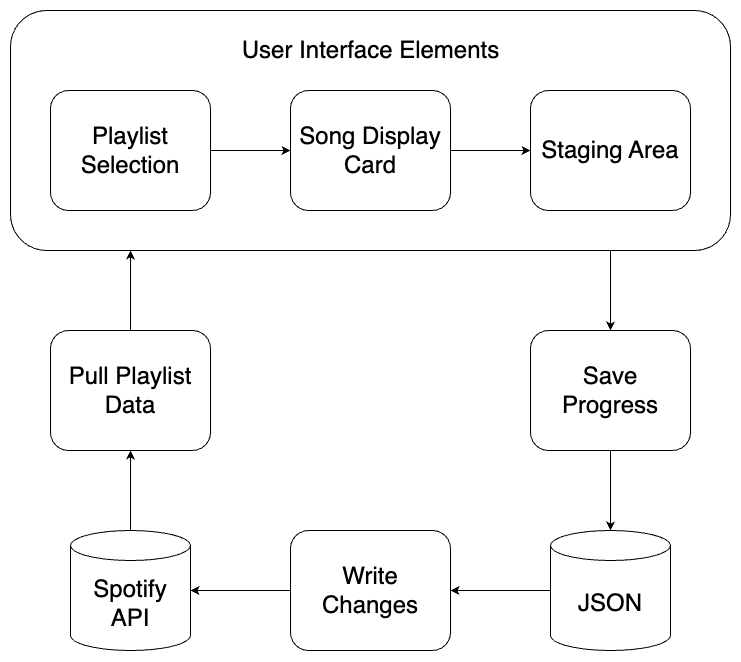
\includegraphics[width=3in]{./arch.png}
  \caption{Architecture diagram}
  \label{fig:architecture_diagram}
\end{figure}

\quad The overall application architecture can be seen in Fig.~\ref{fig:architecture_diagram}. The three major components of our application are the user interface, Spotify API, and a JSON file. The user interface is the core of our application and will perform the majority of functions that we plan to offer. The two main functions of the UI , in accordance with the other major components, are pulling data from the Spotify API and saving progress to a local JSON. The data that is pulled from the Spotify API includes information about playlists and songs. That data is used to prompt the playlist management functions of the UI. The UI also saves the progress of the staging area to a JSON file that is local to the user’s system.\\

\quad The local JSON holds information about the staging area and acts as a cache for that information. It is saved after every action made. This ensures that the user can pick up where they left off. The JSON file is also used in the process of writing changes to the Spotify playlist through the API because it contains the records fo the changes to be made. Once the user finishes managing a playlist, the information for that playlist will be removed from the JSON.

\subsection{User Interface}
\begin{figure}[ht]
  \centering
  \captionsetup{justification=centering}
  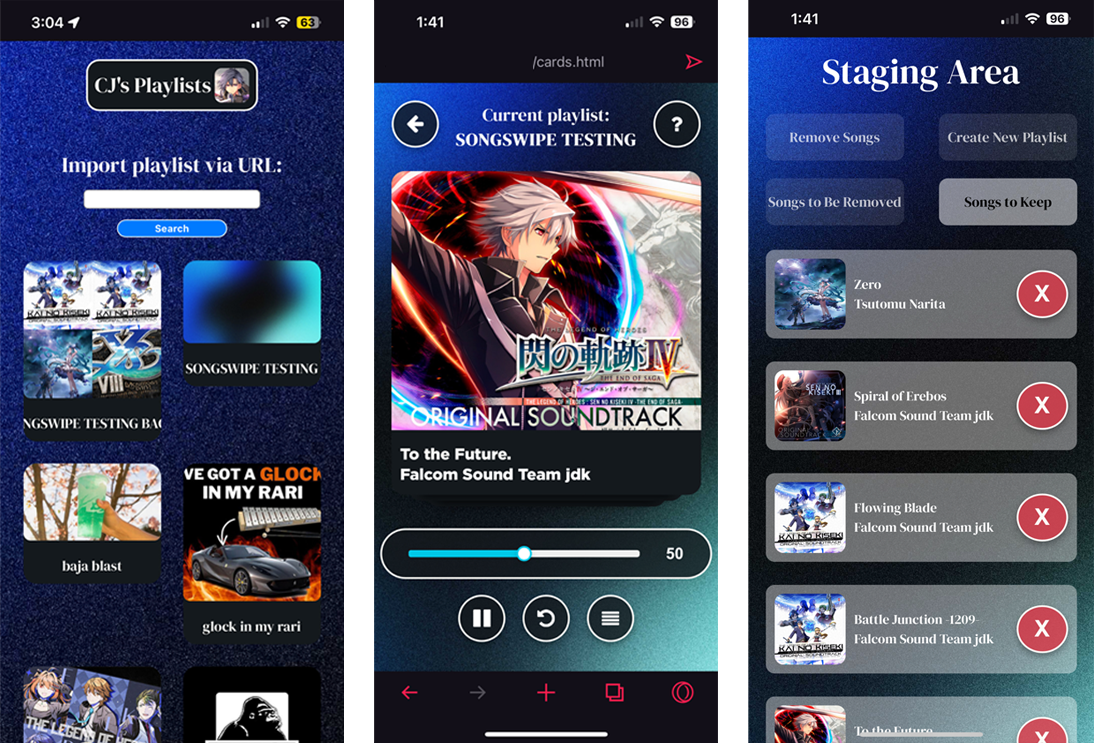
\includegraphics[width=6in,scale=5]{./ui-final.png}
  \caption{Preview of the UI for the playlist selection and card swiping. Left is playlists page, middle is the card swiping screen and the right is the staging area. }
  \label{fig:ui_preview}
\end{figure}

% * <Christopher Coco> 10:52:24 01 Apr 2025 UTC-0400:
% On final paper we should include mocks for all three of the parts, I will include what is currently there.
\quad The user interface consists of three main components: a playlist selection screen, a main swiping screen with cards for each song, and a staging area where any changes can be committed to the Spotify library. The playlist selection screen consists of individual elements showing all user playlists and an area to enter URLs of public playlists. Clicking on a playlist will take you to the card selection screen for that playlist. \\

\quad Once a playlist has been selected, the main swiping screen displays the first song as a large card with the song's information. Users can swipe left or right on each song to decide whether to keep or remove the song from the playlist. Any songs that have been left-swiped will be sent to the staging area to be removed. \\

\quad The staging area shows every song that will be removed from the current playlist.  Users can choose to remove songs from this list if they change their mind.  Once changes have been submitted, meaning that the user can no longer undo changes, it is passed off to a back-end endpoint, where the Spotify API will commit the changes to their library. \\

\subsection{Staging Area Cache}

\begin{figure}[ht]
  \centering
  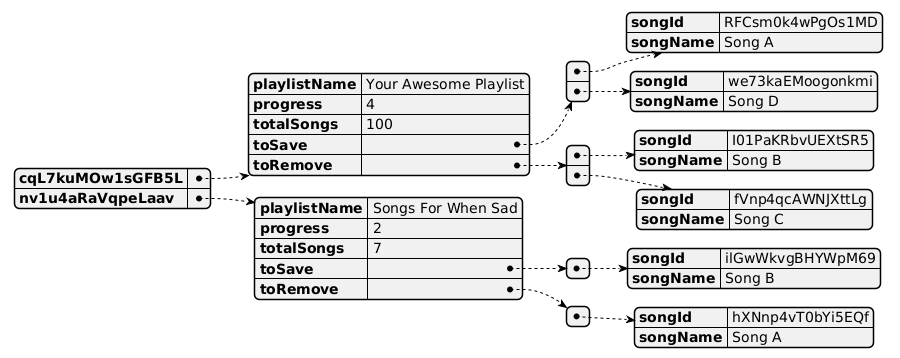
\includegraphics[width=6in]{./json2.png}
  \caption{Visualization of our JSON formatting.}
  \label{fig:jsondiagram}
\end{figure}

\quad When managing a playlist, there is a cache of all the decisions made so far to keep progress. In the case where the application is exited unexpectedly, the progress can be restored. This cache acts as the internal representation of the staging area as well and is read from when changes to the playlist are written. It is stored as JSON on the user’s local storage. Using JSON gives the benefits of easy parsing and setup. An example of the proposed JSON structure can be seen in Fig. ~\ref(fig:jsondiagram). The JSON is partitioned into sections that are determined by the Spotify ID of the playlist. A Spotify ID is a base 62 identifier of an artist, album, track, or playlist \cite{Spotify_docs}. The Spotify ID is guaranteed to be unique for each playlist. Therefore, it is the best way to partition the data because a playlist’s name may change or could have the same name as another playlist. It also can help searching for that playlist again to pick up where you left off. \\

\quad Each playlist has the following attributes defined within it: the playlist name, the progress (amount of songs gone through), the total number of songs, the songs that you have chosen to save, and the songs that you have picked to be removed. The playlist name, progress, and total songs are saved simply just for display purposes. For the choice selection attributes it is a list of objects that hold some information about the songs: the Spotify ID for the song and the name of the song. The Spotify ID is needed for the same reason as the ID for the playlist. The song name is for display purposes. Album cover data is not be cached due to that requiring an image download which will take up unnecessary space on the user’s device. \\

\quad A benefit of using this structure is that it can easily scale. If in the future we decide to update the application to hold more account information this may lead to the use of a database. This structure we defined could easily be added as an attribute in a user record. This would especially work for a non-relational database that follows the document model. \\



\section{Technology Stack}

\subsection{User Interface Technologies}
\quad The user interface is built with the following technologies: HTML, CSS, and Javascript with JQuery \cite{jquery}. This simple, yet effective stack allowed us to make a responsive and effective UI. Using these web development technologies allows SongSwipe to easily be accessible from the web on all platforms. HTML was used to lay out each of the pages for the UI components. CSS was used to stylize the elements that appeared on each of the pages. And finally, Javascript was used to add interactivity to each of the pages. The interactivity includes fetching and writing data from the API service and allowing the user to perform actions. JQuery enhanced adding interactivity by allowing for better event handling and smoother animations. \\ 

\subsection{Spotify API Interactions}
\quad The main technologies used for the backend are Typescript, ExpressJS \cite{expressjs}, and the Spotify API \cite{Spotify_docs}. Typescript was chosen due to its static typing. This minimized type errors with the various data that was worked with. For interacting with the Spotify API, we originally intended to use Spotify's Typescript SDK. However, it was not compatible with the front-end stack that we decided. The library was built to work with technologies like React where the application can be rendered on the server. Our front-end does not support this so we needed to develop a Representative State Transfer (REST) API that acts as a wrapper for the Spotify API. This allows the front-end client to interact with the Spotify API by providing the authorization access token to the REST API endpoints that were developed. It was developed using ExpressJS, a web application framework, that is useful for building REST APIs. The Spotify API as mentioned was used to interact with data on Spotify. One feature that was deprecated from Spotify's API was the ability to get the link to a song's preview. A library \cite{Spotify_preview_url} provided by GitHub user Rexdotsh, provides a workaround for this by extracting the link from Spotify's embed player HTML.

\subsection{Other technologies}
\quad Other technologies that we used involve things related to hosting and unit testing. For a hosting service, we chose Netlify \cite{Netlify}. This is a web hosting platform with a generous free tier and easy integration with GitHub where our repository is hosted. It handles continuous delivery which removes the need for us to configure a deployment pipeline. It also provides 100 GB of bandwidth and 300 build minutes. Netlify's function service \cite{Netlify_functions} was also used. This service allowed the back-end REST API to be hosted in a server-less manner. Netlify functions were also included in the free tier which helps being able to host the site for free. If the application sees success we may need to pivot to a better hosting solution.  We used the Jest library for our Javascript unit testing,it has support for both Javascript and Typescript along with useful features like mocks. Mocks allowed for testing of API endpoints with mock data. Our unit tests were also integrated with our GitHub repository. Whenever a pull request was opened, it could not be merged if any of the unit tests fail. 
%\subsection{Frontend Stack}
%\quad The frontend stack will consist of HTML, CSS, and JQuery. It is a simple, yet effective stack that will allow us to build an effective user interface. Using HTML and web application frameworks will allow SongSwipe to be accessed on all platforms. Our frontend stack will change slightly as the project progresses, as we may add some component libraries or CSS frameworks like Tailwind if we find that they would benefit the usability and look of the UI. \\

%\subsection{Backend Stack}
%\quad For the backend stack, the core programming language that will be used is Typescript. Typescript has better static typing functionality, which minimizes the type of errors that will occur, compared to Javascript; making it a more viable option. SongSwipe will be working with lots of different data and responses from the API, therefore static-type functionality is crucial. Typescript also has a library built by Spotify to help interactions with their Web API, which makes API interaction easier, especially when it comes to Oauth \cite{Spotify_library}. Another important library used in the backend will be extracting song preview URLs from Spotify \cite{Spotify_preview_url}. \\

%\subsection{Other Technologies}
%\quad Netify is a web hosting platform that will host our site. This service allows the app to be easily deployed due to its easy integration with Github, which is used for version control. It also handles continuous delivery, which is beneficial as the hosting service will be integrated with it; removing the need to configure a deployment pipeline. Netify’s free tier is generous and provides up to 100 GB of bandwidth and 300 build minutes \cite{Netify_pricing}. It is perfect for SongSwipe's current state however, if the application seeks wide-scale success then there will be a transition to a scaleable service such as the Cloud, to manage traffic.

\section{Project Challenges}
\quad The main challenges that we had faced was working around the Spotify API which could prove to be tedious at times.  We made use of an external workaround used to get Spotify preview URLs as they no longer support that function by default.  We were initially worried Spotify would deprecate a core feature, however this did not happen.

% \quad The main risks of SongSwipe stem from the potential deprecation of the Spotify API and the risk of the server host, Netlify, changing its free-to-use terms. These updates happen all of the time, meaning if SongSwipe were using a deprecated function, it would break the app. Not only that but if Netify ceases its free-to-use terms, the app will be unavailable. Furthermore, if someone uses the application after a security fix it might put the user at risk of a major security vulnerability.  \\

% Over a short period of time, the Spotify API deprecates features randomly which can cause issues during development. Whereas if a feature is used for SongSwipe's core functionality, then the app will break. For example last November, a few features were removed from the API which include: related artists, recommendations, audio features, audio analysis, access to algorithmically generated and Spotify-owned editorial playlists, and 30-second preview URLs in ‘muli-get’ responses \cite{Spotify_api_removal}. There is also a chance that the current features of the Spotify API could have bugs. For example, a bug with the preview urls made it always return a null value instead of what was needed \cite{Spotify_preview_url}. If a bug is encountered using the API, with no current solution to solving the bug, that would result in dawdling which will cut back on the timeline of the our milestones. Deprecation will always be a huge risk in development that could affect the application's usability. Therefore it is SongSwipe's high priority to always read API updates and documentation.

% \section{Milestones}
% \quad For our project, we plan to split up our project into milestones that will be accomplished on a weekly basis starting on February 21st. These will essentially mimic sprints and at the start of each sprint we will break each milestone into the parts that need to be completed. We have seperated milestones between front and back end. This schedule is subject to change depending on issues that we run into during development. 

% \begin{itemize}
%     \item \textbf{April 4th, 2025:}
%         \begin{itemize}
%             \item \textbf{Frontend:} Make homepage and a playlist search bar.
%             \item \textbf{Backend:} Pull preview URLs for songs and populate card swiping screen.
%         \end{itemize}
%     \item \textbf{April 11th, 2025:}
%         \begin{itemize}
%             \item \textbf{Frontend:} Adjustments to make app compatible on desktop.
%             \item \textbf{Backend:} Allow for writing to Spotify playlists. 
%         \end{itemize}
%     \item \textbf{April 18th, 2025:}
%         \begin{itemize}
%             \item Final submission preparations and usability testing.
%         \end{itemize}
%     % \item \textbf{May 2nd, 2025} - it will probably be due by this idk if we should have it
% \end{itemize}

\section{Unit Testing}
\quad \quad We used Jest for our unit tests.  They were broken up into four different units: API endpoints, Spotify interactions, Spotify preview request, and utility functions. The API endpoint testing checked to see if each endpoint on our REST API responded with the correct status codes and body. We used Jest's mock functionality to mock data returned from Spotify's API. This allowed us to insert mock data with a similar structure to what was expected from Spotify's API to ensure correct data was returned when successful. For testing related to Spotify interactions, tests covered the functions that dealt with formatting requests and checking responses for any errors. This ensured that there were no errors from us in sending the requests. For testing the Spotify preview library, the test makes sure that the correct fetch is called to ensure that if the library is updated it still works as it needs to. We also created tests for our utility functions, such as creating random keys when calling Spotify API.

\section{User Usage Metrics Collection}
\quad One feature we added to our application to test usage efficiency is metric collection. Based on a toggle in the .env file for the project, metrics collection can be enabled. When enabled, whenever a user goes to edit a playlist a csv and text file will be created to append data to. The csv file will contain the song name, artist, album, the time to make a decision in seconds, and the decision made for all of the songs in the users playlist that they went through. The text file will contain the total amount of time it took for the user to go through the playlist. Having this data ensures that we have accurate metrics on how our application performed, which were used to judge effectiveness. For collecting metrics for Spotify we made it easier by writing a Python script that waits for input to indicate a decision and keeps track of the time between decisions. When using this script the decision was logged once the user went to the next song. This data was then written to a csv file. 

\section{Usability Testing}
\quad To validate our project and its ability to solve the proposed problem, we conducted two types of tests, each targeting one of the application's primary use cases: managing personal Spotify playlists and copying playlists from other users. Our goal for this testing is to directly compare the same task performed with both the Spotify UI, as well as SongSwipes. In our individual unmeasured testing, we could feel the improvement, however we wanted to quantify it.

\subsection{Estimation}
\quad As reviewed previously in our presentation, we decided to give an estimation of our product and how it could save you time. \\

When regarding Spotify, once a song is inside a playlist, you could no longer listen to the preview unless you find the source by searching the song on the platform. Therefore, this makes Spotify playlist revision significantly tedious because you would have to listen to the song, or determine the most popular part of the song, usually the chorus, and then formulate whether you like the song or not, then remove the song through Spotify’s tedious song removal process. \\

We deducted that the process of reviewing songs in a playlist, with regards to Spotify, would take about 30 seconds for each song and another 3 seconds to remove user selected songs. In regards to SongSwipe, we deducted that it would take 15 seconds to review each song and another second to swipe. At the time of this estimation, we only calculated Spotify Premium users.

\begin{center}
Given that $x$ is the number of songs in a playlist and $y$ is the number of songs you want to remove. The estimation equation will look like this:
\end{center}
\begin{equation}
30 \text{ seconds} \times x + 3 \text{ seconds} \times y = \text{Time Consumption Estimation for Spotify}
\end{equation}
\begin{equation}
15 \text{ seconds} \times x + 1 \text{ seconds} \times y = \text{Time Consumption Estimation for SongSwipe}
\end{equation}
\subsection{Procedure}
    For our testing, we decided to test multiple methods to encapsulate all the different kinds of users that would be using our application. \\

    For testers, we selected people who first had Spotify. It would take more time to teach someone how to navigate Spotify UI testing, compared to someone who was more familiar to it. They also needed some patience to follow the procedure correctly when asked. Finally, they had to be someone who was willing to spend a good chunk of time testing both the Spotify UI and our SongSwipe UI free of charge because we are too broke to pay for people who were specifically trained to test these types of applications.

\subsubsection*{Method A}
For this method, we wanted to target the most common user who would be using our application, which would be:\\
    
Someone who plays their playlist on shuffle and skips songs they no longer like, yet still have the song in the playlist, we have implemented the procedure as follows: \\

   \textbf{Controlled Environment:}
    
    \begin{itemize}
    \item \textbf{Playlist:} Standard playlist consisting of 75 songs
    \item \textbf{Target Artist:} Pitbull (9 songs in the playlist)
    \item \textbf{Listening Time:} 5 seconds per song
    \end{itemize}
    
    \textbf{Spotify Testing:} 
    
    \begin{enumerate}
        \item Play the playlist on shuffle mode
        \item Locate the chorus and listen to the song for 5 seconds
        \item After the 5-second listening period:
            \begin{itemize}
                \item If artist is not Pitbull: Skip the song
                \item If artist is Pitbull: Remove the song from the playlist
            \end{itemize}
    \end{enumerate}

    \textbf{SongSwipe Testing:}
    
    \begin{enumerate}
        \item Listen to each song for the mandatory 5-second period
        \item After the 5-second listening period:
            \begin{itemize}
                \item Testers are only permitted to swipe left when the artist is Pitbull
                \item All other artists should not be swiped left
            \end{itemize}
    \end{enumerate}

    Both Spotify UI and our SongSwipe UI have text to show the song and artist, which makes the selection accessible both audibly and visually.

\subsubsection*{Method B}

For this method, we wanted to targest the other use case of our application going through a friends playlist and selecting songs that you like.

Both Spotify UI and our SongSwipe UI have text to show the song and artist, which makes the selection accessible both audibly and visually.
    
Before beginning these tests, the participants had the use cases of our application explained along with their task. Music for the playlists were also tailored to be music that the participant would not know.

    \textbf{Controlled Environment:}
    
    \begin{itemize}
    \item \textbf{Playlist:} Two different playlists with 50 songs that were all different.
    \item \textbf{Task Assigned:} Listen to music for however long you choose and make a decision if you like it or not.
    \end{itemize}

    \textbf{Spotify Testing:} 
    
    \begin{enumerate}
        \item Play the playlist on shuffle mode.
        \item List to song for amount of time that is up to the user.
        \item After decision is made:
            \begin{itemize}
                \item If they like it: Add playlist like shown in Fig.~\ref{fig:spotify_diagram}
                \item If they did not like it: Skip song
            \end{itemize}
    \end{enumerate}

    \textbf{SongSwipe Testing:}
    
    \begin{enumerate}
        \item Listen to the preview of song for however long.
        \item After listening:
            \begin{itemize}
                \item Swipe right if they liked the song
                \item Swipe left if they disliked the song
            \end{itemize}
    \end{enumerate}

\section{Reporting Results}

\subsection*{Tables}
Method A
\begin{longtable}{lllll}
Tester Name & Spotify Subscription & Spotify Time & SongSwipe Time \\
\hline
TesterA & Free User & $\leq$ 3 hours 2 minutes & 6 Minutes 25 Seconds \\
TesterB & Spotify Premium & 42 minutes and 5 Seconds & 13 Minutes and 38 Seconds \\
\end{longtable}

% FIX IT BEING INDENTED
Method B
\begin{longtable}{lllll}
    Tester Name & Spotfy Time & SongSwipe Time & Spotify Average & SongSwipe Average \\
    \hline
    TesterA & 13.03 minutes & 8.1 minutes & 15.64 seconds & 9.72 seconds \\
    TesterB & 5.92 minutes & 4.08 minutes & 5.76 seconds & 7.1 seconds \\
\end{longtable}

% Same with the method b thing
\subsection*{Figures}

Fig~\ref{fig:methodbstats}

\begin{figure}[ht]
    \centering
    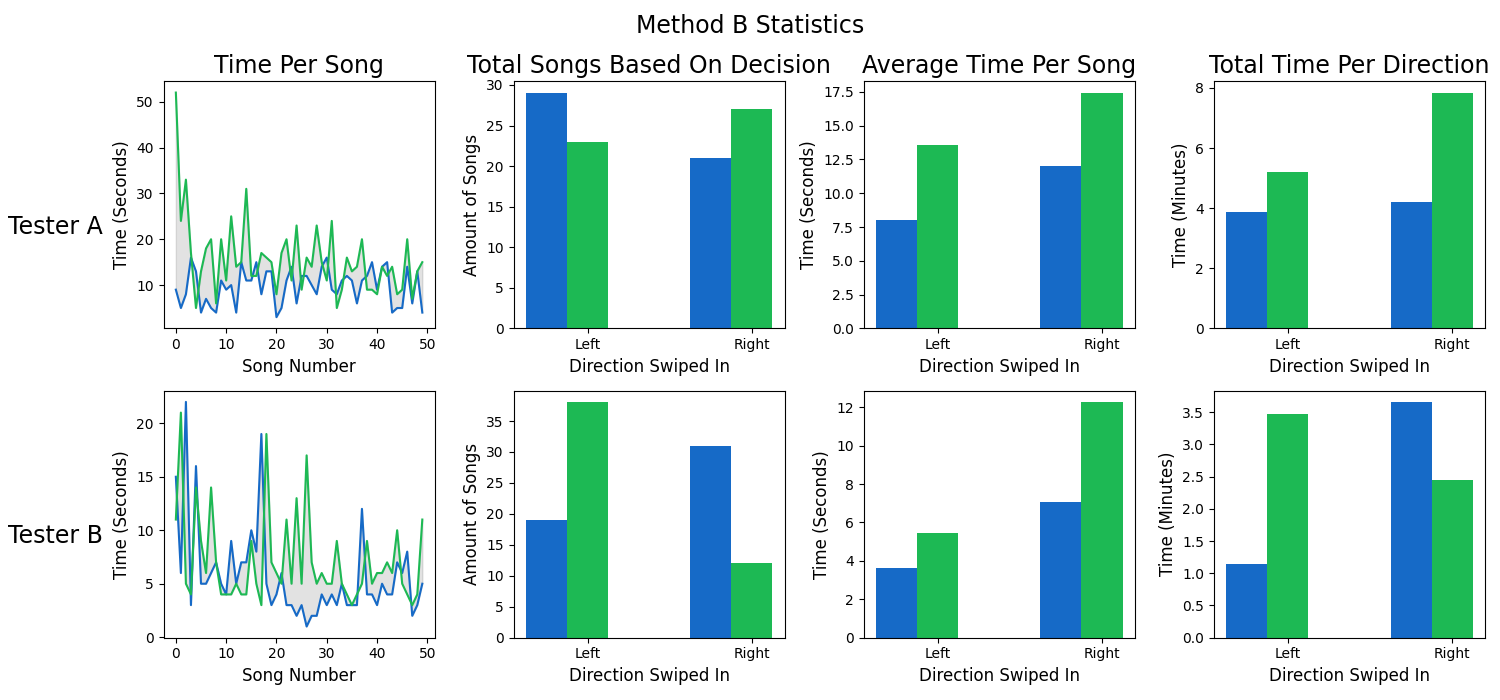
\includegraphics[width=6in]{./method_b_statistics.png}
    \caption{Statistics for Method B. Includes time per song, total songs based on decision, and total and average times. Generated using Matplotlib \cite{Matplot}.}
    \label{fig:methodbstats}
  \end{figure}

\subsection{Limitations}
When it comes to testing, there will always be some form of limitations. In our project, to scope the most data we can get, we had all the members conduct their own testing with their own procedure, and by doing this,s we would have different results based on the guidelines in their respective procedures.

Spotify limits the number of skips a free user can have, about 6 skips every hour. Tester A, who is a free user, attempted to conduct the test; it was too tedious and time-consuming so we decided to perform an approximation on how long it would take. After realizing free Spotify users exist, this demonstrates that our application will greatly reduce time consumption in the decision-making process as our users will only have to listen to the song for at most 15 seconds per song.
    
\begin{center}
    We calculated the Spotify approximation based on the amount of hours it will take to listen to the whole playlist from start to finish. We also deducted that a skip will approximately save a person 4 minutes as a song can range from 3-5 minutes, so 4 is the middle ground. \newline 
\begin{equation}
\text{Total Playlist Time} - \lfloor\text{Listening Hours}\rfloor \times 6\text{ skips/hour} \times 4\text{ minutes} = \text{Spotify Consumption Approximation}
\end{equation}
\end{center}

\subsection{Discussion}

\subsection*{Method A}
Based on our experiment, we had 75 songs in our playlist, which had a total listen time of 4 Hours and 38 Minute,s and we removed 9 songs from that playlist. \\
    
Using our Estimation equations above (1 and 2), we estimated that it would take 37 Minutes and 57 Seconds for Spotify and 19 Minutes and 54 Seconds for SongSwipe. This has a time reduction of 47.5\%. It is observed that the more songs are in a playlist, the time spent on playlist management is significantly reduced.\\
    
When looking at our actual results from user testing, we see that TesterA has about a 95\% time reduction meanwhile TesterB has a 67.8\% time reduction. This shows that our application goes beyond our expectations by showing a time reduction of more than 50 \% and even more when it comes to free Spotify users, who have harsh limitations on song skips. \\

\subsection*{Method B}
Based on the experiments for method B, it can be seen that SongSwipe has a clear advantage when it comes to the time spent. \\

% Maybe include the formula for the percentage difference.
Adding together the total times for both testers for Method B makes the percentage difference in total time 43\%. Doing the same for average time brings the percentage difference to 65\%. This shows that for going through new music quickly, SongSwipe can aid in that process and lower the time spent. \\

Some other trends were noticed in testing with the users. For both testers, it was noticed that there was visable frustration when messing up an input on Spotify's client and sometimes getting annoyed when they could not find the playlist to add the song to. While using SongSwipe this was not observed.

Another trend that happened was that the testers did not really scrub through the song at all while using Spotify. This might have been due to them doing SongSwipe first which shows that there is more of a quick nature to it. More testing could have been done where Spotify was used first to see if this made any impact at all.

% Maybe a conclusions section

\section{Lessons Learned}

Through this project, we learned a lot of valuable lessons in architecting and developing a solution to a problem and how to work as a team. Throughout the semester, we revised and improved the original idea for the project based on the various feedback we received from our professor and peers. This made us rethink different aspects of our application and helped sharpen our ideas. \\

We also improved a lot at sharing our ideas. Writing multiple papers throughout the semester has helped. It forced us to think about how we can share our ideas in a way that makes sense. It made us think more about whether we needed certain things if we were overthinking something. It also had us present aspects of our application through diagrams, which helped with development. \\

For technical lessons learned, we learned a lot about designing a web application without the more modern tools that are typically used today. This was a nice change of pace and made us think about challenges that are typically solved with the libraries. An example of this would be routing; instead of using a nice routing library, we had to do routing ourselves and use pattern matching to make sure that the application would behave the same if it was being run locally or on a hosting service. We also learned a lot about OAuth and having to manage the lifetimes of authorization tokens due to not being able to utilize the Spotify Typescript SDK. This also allowed us to work more with REST APIs and design endpoints to interact with Spotify.

% Start the appendix
\begin{appendices}
    \renewcommand{\thesection}{Appendix \Alph{section}:}
\section{Contributions}
\begin{itemize}
     \item \textbf{Anthony Simao:}
        \begin{itemize}
            \item Front-end development, HTML, and CSS for page styling and basic animations.
            \item Back-end development, JavaScript, and jQuery for basic event handling and animations.
        \end{itemize}
    \item \textbf{Nena Heng:}
        \begin{itemize}
            \item Front-end development, focusing on CSS styling to ensure a user-friendly GUI.
        \end{itemize}
    \item \textbf{Christopher Coco:}
        \begin{itemize}
            \item Back-end development in Typescript involves Spotify API calls and credential management, unit testing, and deployment
        \end{itemize}
    \item \textbf{Katiana Sourn:}
        \begin{itemize}
            \item Back-end development regarding local storage, expected behavior configuration, and back-end UI handling
            \item Assisting with Spotify API calls
        \end{itemize}
    \item \textbf{Raj Ray:}
        \begin{itemize}
            \item QA Tester
        \end{itemize}      
\end{itemize}
\section{Feedback}
\quad We received several important pieces of feedback from our instructor to improve the goals and specifications of the project. The UI functionality and button pressing have been addressed in our proposal in terms of explaining what each button is and does exactly as that was not clear before. The project risk of using the Spotify API now includes clear-cut examples that occurred in recent months, such as features that were added and removed. The described features explain how they can affect the core functionality of our project. The metric of finger travel distance has been reworded. Instead of using this specific metric, we explained the core problem using the number of required button presses. \\

After receiving peer reviews, we revised our project proposal. Our peers stressed the risks of using Spotify API because of deprecations. We as a team, are aware of possible issues with this and have taken it into account with what we want for our software. Previews were also a main concern by our peers, considering the nature of how they work. They play an essential part in our project in helping the user determine if they would like to remove a song or not. In terms of the proposal itself, each team member has thought about how we word certain specifications and concepts to best fit our audience. We've also added diagram captions to better explain the figures in our proposal. We have taken both peer and professor advice and detailed the milestones for every week and separated them as backend and frontend milestones. As it was not clear before, we've also explained what each piece of technology clearly does and will provide for our project specifically.s

\end{appendices}

% \begin{figure}[h]
%     \centering
%     \begin{minipage}{0.2\textwidth} % Adjust width as needed
%         \centering
%         \includegraphics[width=\textwidth]{1.jpeg}
%     \end{minipage}
%     \hspace{2cm} % Adjust space between images
%     \begin{minipage}{0.2\textwidth}
%         \centering
%         \includegraphics[width=\textwidth]{2.jpeg}
%     \end{minipage}
%     \caption{Main swipe screen and song staging area mockup.}
% \end{figure}

% \section{Bibliography}
% \begin{enumerate}[label={[\arabic*]}]
%     \item \textit{Playmixify}, https://playmixify.com/
%     \item \textit{Skiley}, João Vitor Verona Biazibetti, https://skiley.net/
%     \item \textit{Spotify Dedup}, JMPerez, https://Spotify-dedup.com/
%     \item \textit{Spotify Removes Features From Web API Citing Security Issues}, Stuart Dredge, November 2024, https://musically.com/2024/11/28/Spotify-removes-features-from-web-api-citing-security-issues/
%     \item \textit{Spotify Preview URL}, Rexdotsh (Github User), 2025, https://github.com/rexdotsh/Spotify-preview-url-workaround?tab=readme-ov-file
%     \item \textit{Swipefy}, Swipefy B.V,  https://swipefy.app/
%     \item \textit{Spotify User Statistics 2025}, Shubham Singh, https://www.demandsage.com/Spotify-stats/
% \end{enumerate}
\begin{thebibliography}{9}

\bibitem{SongSwipe} Christopher Coco, Nena Heng, Raj Ray, Anthony Simao, Katiana Sourn, \textit{SongSwipe} Available: \url{https://github.com/ListenToAJ/SongSwipe}

\bibitem{Spotify_stats} Shubham Singh. “Spotify User Statistics 2025.” Available: \url{https://www.demandsage.com/Spotify-stats/}

\bibitem{Spotify_app} Spotify. \textit{Spotify App}. Available: \url{https://www.spotify.com/}

\bibitem{Spotify_docs} Spotify. \textit{Web API Documentation}, Available: \url{https://developer.spotify.com/documentation/web-api}

\bibitem{Spotify_library} Spotify. \textit{Web API TS SDK}, Available: \url{https://github.com/spotify/spotify-web-api-ts-sdk}

\bibitem{playmixify} Playmixify. Available: \url{https://playmixify.com/}

\bibitem{skiley} João Vitor Verona Biazibetti. Skiley. Available: \url{https://skiley.net/}

\bibitem{Spotify_dedup} JMPerez. Spotify Dedup. Available: \url{https://Spotify-dedup.com/}

\bibitem{Spotify_api_removal} Stuart Dredge. “Spotify Removes Features From Web API Citing Security Issues,” November 2024. Available: \url{https://musically.com/2024/11/28/Spotify-removes-features-from-web-api-citing-security-issues/}

\bibitem{Netlify} Netlify, Available: \url{https://www.netlify.com}

\bibitem{Netlify_functions} Netlify Functions, Available: \url{https://www.netlify.com/platform/core/functions/}

\bibitem{Netlify_pricing} Netlify Pricing. \textit{Serivce Pricing}, Available: \url{https://www.netlify.com/pricing/}

\bibitem{Spotify_preview_url} Rexdotsh. “Spotify Preview URL,” 2025. Available: \url{https://github.com/rexdotsh/Spotify-preview-url-workaround?tab=readme-ov-file}

\bibitem{swipefy} Swipefy B.V. Swipefy. Available: \url{https://swipefy.app/}

\bibitem{drawio} Draw.io, Available: \url{https://draw.io/}

\bibitem{jsonuml} PlantUML JSON Diagrams, Available: \url{https://plantuml.com/json}

\bibitem{jquery} Jquery, Available \url{https://jquery.com/}

\bibitem{expressjs} ExpressJS, Available \url(https://expressjs.com/)

\bibitem{Jest} Jest, Available \url(https://jestjs.io)

\bibitem{Matplot} Matplotlib, Available \url{https://matplotlib.org/}


\end{thebibliography}


\end{document}


%% Rylie swiping with 5 seconds in between: 6 minutes 25 seconds

% %% Any changes made since

% %% Define success for SongSwipe

% %% Estimation of Results

% %% Make a random playlist of different sizes

% %%  - Pick songs you want to remove
% %%  - Record time it takes to remove via mobile/PC
% %%  - Follow the same procedure using SongSwipe via mobile/PC

% %% Make a table to show results

% %% Maybe make an equation to estimate time usage of regular Spotify UI vs SongSwipe

% %% Describe unit test and why they are needed